\documentclass[10pt, conference, compsocconf]{IEEEtran}
% \documentclass[conference]{../sty/IEEEtran}
%\usepackage{ifpdf}
%\usepackage{cite}
\ifCLASSINFOpdf
  \usepackage[pdftex]{graphicx}
  \graphicspath{{./images/}}
\else
  \usepackage[dvips]{graphicx}
  \graphicspath{{./images/}}
\fi
%\usepackage[cmex10]{amsmath}
%\usepackage{algorithmic}
\usepackage{array}
\usepackage{amsmath}
\usepackage{supertabular}
%\usepackage{mdwmath}
%\usepackage{mdwtab}
%\usepackage{eqparbox}
%\usepackage[caption=false]{caption}
%\usepackage[font=footnotesize]{subfig}
%\usepackage[caption=false,font=footnotesize]{subfig}
%\usepackage{fixltx2e}
%\usepackage{stfloats}
%\usepackage{url}
%\hyphenation{op-tical net-works semi-conduc-tor}

\begin{document}

\title{A Compact Implementation of the AES Encryption/Decryption based on Composite Glois Field}



\author{\IEEEauthorblockN{
Abhishek Bajpai\IEEEauthorrefmark{1},
Shubhamoy Maitra\IEEEauthorrefmark{2},
%Sunil Kulgod\IEEEauthorrefmark{2}
%S K Parulkar\IEEEauthorrefmark{4},
%R S Mundada\IEEEauthorrefmark{5}
}
%\IEEEauthorblockA{Computer Division,
%Bhabha Atomic Research Centre,\\
%Mumbai, India\\
%Email: (
%\IEEEauthorrefmark{1}abbajpai, 
%\IEEEauthorrefmark{3}bathebn, 
%\IEEEauthorrefmark{2}svkulgod%, \\ 
%\IEEEauthorrefmark{4}skparul, 
%\IEEEauthorrefmark{5}rsm
%)@barc.gov.in}
\and
\IEEEauthorblockN{
%Jayant Sharma\IEEEauthorrefmark{6},
%Diksha Moolchandani\IEEEauthorrefmark{7}, \\
%Deepak Kapoor\IEEEauthorrefmark{8}, 
%Rahul Yamasani\IEEEauthorrefmark{9}%,
%Saket Saurav\IEEEauthorrefmark{10}
}
%\IEEEauthorblockA{IIITDM Jabalpur,
%India\\
%Email: (
%\IEEEauthorrefmark{6}jayantsharma, 
%\IEEEauthorrefmark{7}dikshamoolchandani,\\ 
%\IEEEauthorrefmark{8}deepakkapoor, 
%\IEEEauthorrefmark{9}yamasanirahul%, 
%%\IEEEauthorrefmark{10}saket
%)@iiitdmj.ac.in}
}

% use for special paper notices
%\IEEEspecialpapernotice{(Invited Paper)}

\maketitle



\begin{abstract}
There have been several implementations of compact AES encryption/decryption cores in terms of gate area. Generally optimistaions are based on implementing Substitution box in a sub galois field. In this proposal we would like to investigate wether we can implement complete AES round including shift row, mix column and add round key in sub galois field domain. Assumption is that we can have mix column in sub galois field as compact as present mix column and further better optimised inverse mix column in sub galois field. If this assumption is correct then we can straight away avoid $GF(2^8) \leftrightarrow GF((2^4)^2)$ transformations at every round while doing substitution byte.

\end{abstract}

\maketitle



%%%%%%%%%%%%%%%%%%%%%%%%%%%%%%%%%%%%%%%%%%%%%%%%
%% SECTION
%%%%%%%%%%%%%%%%%%%%%%%%%%%%%%%%%%%%%%%%%%%%%%%%
\section{Introduction}
In 2001 Rijndael design was established as the Advanced Encryption Standard (AES) for the encryption of electronic data by the U.S. National Institute of Standards and Technology (NIST). Since then Rijndael design has been subject to several cryptanalysis and till date no serious attacks have been found. There have been lot of efforts also for an optimised implementation of this algorithm in software as well as hardware.

In this proposal we will study sub galois field based optimisation approaches for implementing AES algorithm and we will see wether we can extend it to the other blocks of the algorithm in order to have better compact core. We will also study shared features of encryption and decryption cores in sub galois field domain. Further we would like to have implementations optimised for Area/Speed and both as well.

%%%%%%%%%%%%%%%%%%%%%%%%%%%%%%%%%%%%%%%%%%%%%%%%
%% SECTION
%%%%%%%%%%%%%%%%%%%%%%%%%%%%%%%%%%%%%%%%%%%%%%%%
\section{AES Algorithm}
The AES algorithm, also called the Rijndael algorithm, is a symmetric block cipher, where the data is encrypted/decrypted in blocks of 128 bits. Each data block is modified by several rounds of processing, where each round involves four steps. Three different key sizes are allowed: 128 bits, 192 bits, or 256 bits, and corresponding several rounds for each is 10 rounds, 12 rounds, or 14 rounds, respectively. From the original key, a different "round key" is computed for each of these rounds. For simplicity, the discussion below will use a key length of 128 bits and hence 10 rounds.

\begin{figure}
  \centering
    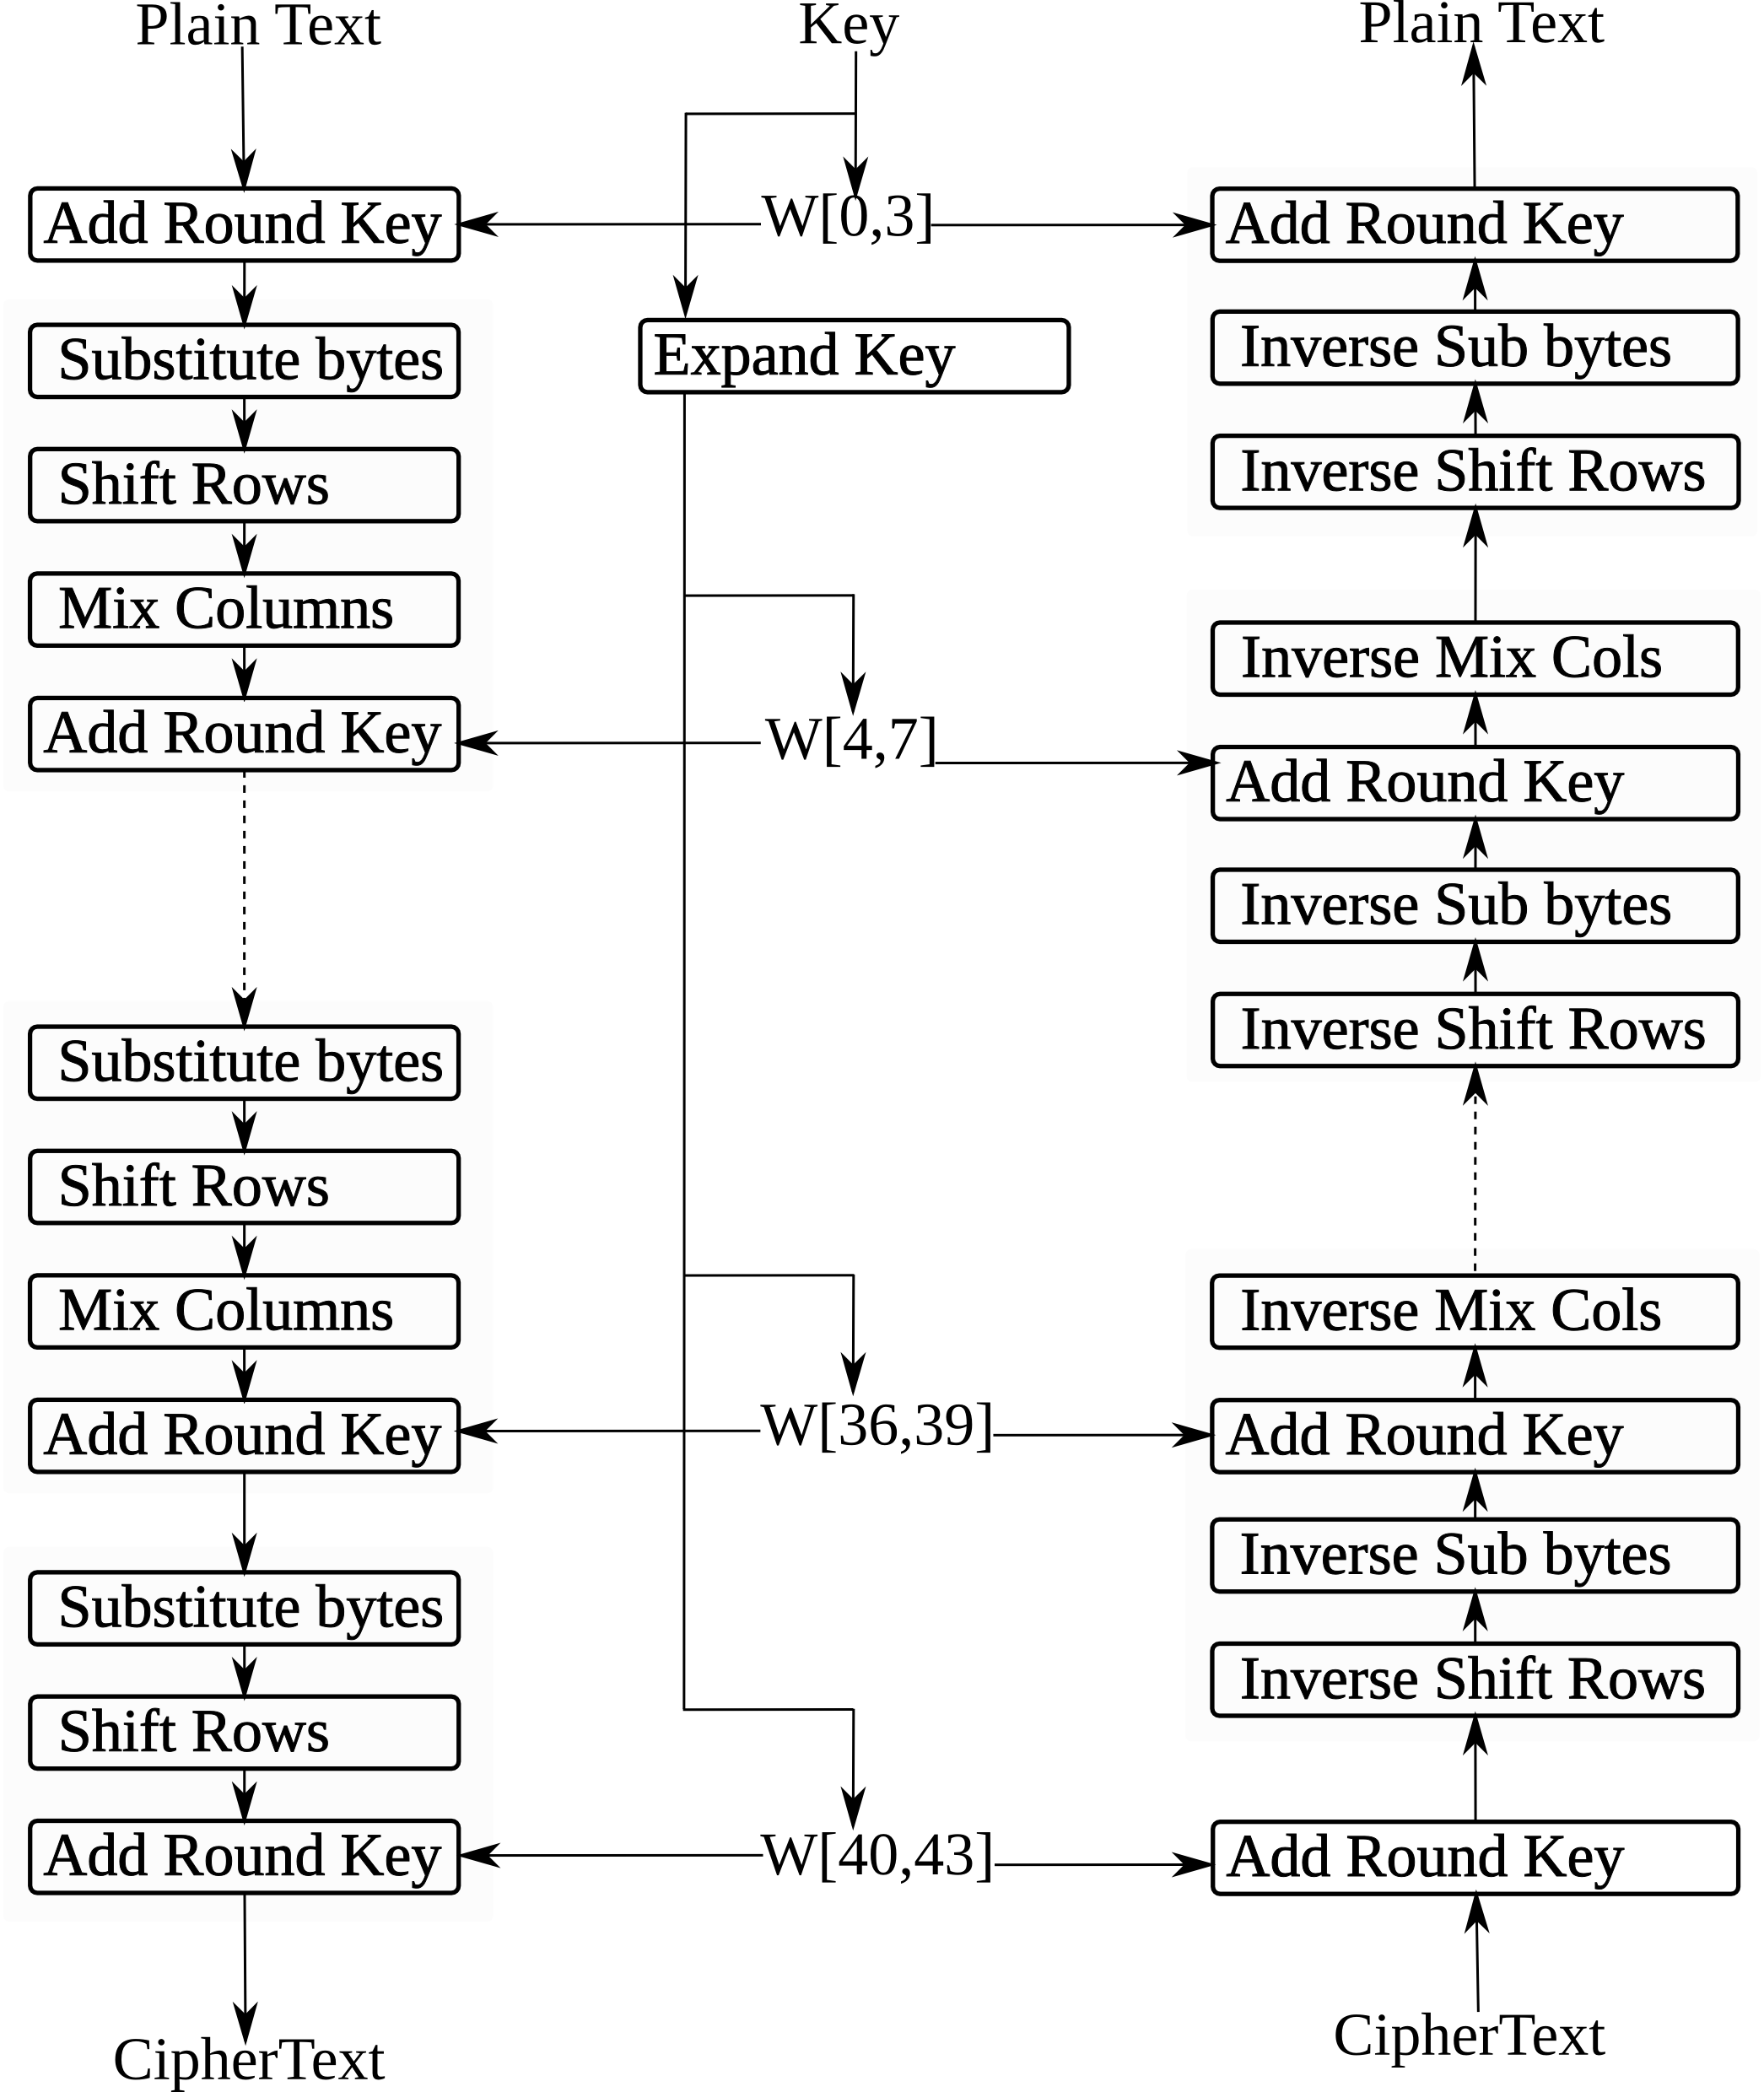
\includegraphics[width=0.50 \textwidth]{images/AES_structure.png}
  \caption{AES Algorithm Flow Diagram\cite{Processing_announcingthe}}
  \label{AES_structure}
\end{figure}

    Their are four steps in each round of encryption, in order, they are called SubBytes (byte substitution), ShiftRows, MixColumns, and AddRoundKey. Before the first round, the input block is processed by AddRoundKey. Also, the last round skips the MixColumns step. Otherwise, all rounds are the same, except each uses a different round key, and the output of one round becomes the input for the next. For decryption, the mathematical inverse of each step is used, in reverse order; certain manipulations allow this to appear like the same steps as encryption with certain constants changed. Each round key calculation also requires the SubBytes operation. (More complete descriptions of AES are available from several sources, e.g., \cite {Processing_announcingthe})

    Of these four steps, three of them (ShiftRows, MixColumns, and AddRoundKey) are linear, in the sense that the output 128-bit block for such steps are just the linear combination of the outputs for each separate input bit.

    The single nonlinear step is the SubBytes step, where each byte of the input is replaced by the result of applying the "S-box" function to that byte. This nonlinear function involves finding the inverse of the 8-bit number, considered as an element of the Galois field $GF(2^8)$. The Galois inverse is a complex function, and so many current implementations use a table of the S-box function output. This table look-up method is fast and easy to implement as far as software is concern.
    
    But for hardware implementations of AES, table look-up approach for the S-box function is too much area consuming. Each of the 16 bytes in a block can go through the S-box function independently, and so could be processed in parallel for the byte substitution step. This effectively requires 16 copies of the S-box table for one round. To fully pipeline the encryption would entail "unrolling" the loop of 10 rounds into 10 sequential copies of the round calculation. This would require 160 copies of the S-box table (200 if round keys are computed "on the fly"), a significant allocation of hardware resources.


\section{Byte Substitution}\cite{BerkSunar}
The Byte Substitution transformation operates independently on each byte of the state. The operation comprises of 2 sub-steps:  
\begin{enumerate}
\item Inversion: Multiplicative inverse of each byte is taken in $GF(2^8)$, and \{00\} is mapped to itself.
\item Affine Transformation: This sub-step is performed in GF(2).
\end{enumerate}

To implement the Byte Substitution transformation, many techniques have been reported. Those are, for instances; 

\begin{enumerate}
\item The table lookup technique where step 2 is usually combined into a single table known as S-box. Not feasible as discussed.
\item Synthesis and optimized logic function of S-box using CAD tools, and 
\item Compute inversion of element in $GF(2^8)$ and optimize the logic functions. The efficiency of the third technique is much depended on the mathematical theory of field element inversion. This approach is highly considered when the table lookup is not applicable or when the compact design is a case. It also provides desirable features for the highly paralleled computation.
\end{enumerate}

In this proposal we will be studying option (3) since the field inversion hardware can be easily shared by both the encryption process and decryption process. The Byte Substitution (and similarly, the inverse Byte Substitution) transform of a byte is defined mathematically as:

\begin{equation}
D(x) = \delta  A^{-1} (x)_{mod (x^8 + 1)} \oplus C(x)
\end{equation}


where $C(x)~=~x^6~+~x^5~+~x~+~1~=~\{63\}$ and $\delta~=~\{1F\}~=~x^4~+~x^3~+~x^2~+~x~+~1$. For the inverse Byte Substitution computation, $\delta~=~\{4A\}~=~x^6~+~x^3~+~x$ and $C(x)~=~x^2~+~1~=~\{05\}$ are used respectively. The constant C(x) has been added so that the Sbox has no fixed point (a map to a) and no opposite fixed point ( a map to \={a} ). Besides the field inversion. 



%%%%%%%%%%%%%%%%%%%%%%%%%%%%%%%%%%%%%%%%%%%%%%%%
%% SUBSECTION
%%%%%%%%%%%%%%%%%%%%%%%%%%%%%%%%%%%%%%%%%%%%%%%%
\subsection{$GF(2^8)$ to $GF((2^4)^2)$ transformation\cite{springerRudra}\cite{1149067}}
   AES has adopted $m(x) = x^8 +x^4 +x^3 +x+1$ as its field polynomial. Although such a polynomial is an irreducible but it is not a primitive one. Fortunately, with the field isomorphism property, we can map elements in $GF(2^8)$ as shown in [4] to the composite field $GF((2^4)^2)$ based on the polynomial $w(x)=x^2+x+ \beta ^{14}$ , where $\beta ^{14}=\{09\}$ denotes the element in $GF(2^4)$ of which $I(x) = x^4 + x + 1$ is the primitive irreducible polynomial. Let D be an element in $GF(2^8)$ and A be an element in $GF((2^4)^2)$ , then $A = [T] D$ and $D = [T]^{\_ 1} A$
   
where
\begin{equation}
T = \left[ \begin{array}{cccccccc}
1 & 0 & 1 & 1 & 1 & 0 & 1 & 1 \\
0 & 1 & 0 & 1 & 0 & 0 & 0 & 0 \\
0 & 1 & 0 & 0 & 1 & 0 & 1 & 0 \\
0 & 1 & 1 & 0 & 0 & 0 & 1 & 1 \\
0 & 0 & 0 & 0 & 1 & 1 & 1 & 0 \\
0 & 1 & 0 & 0 & 1 & 0 & 1 & 1 \\
0 & 0 & 1 & 1 & 0 & 1 & 0 & 1 \\
0 & 0 & 0 & 0 & 0 & 1 & 0 & 1 \\
 \end{array} \right] 
\end{equation}
and
\begin{equation}
T^{-1} = \left[ \begin{array}{cccccccc}
1 & 0 & 0 & 0 & 1 & 0 & 1 & 0 \\
0 & 0 & 0 & 0 & 1 & 1 & 0 & 1 \\
0 & 1 & 0 & 0 & 1 & 1 & 1 & 0 \\
0 & 1 & 0 & 0 & 1 & 1 & 0 & 1 \\
0 & 1 & 0 & 1 & 1 & 0 & 1 & 0 \\
0 & 0 & 1 & 0 & 0 & 1 & 0 & 1 \\
0 & 1 & 1 & 1 & 0 & 1 & 1 & 1 \\
0 & 0 & 1 & 0 & 0 & 1 & 0 & 0 \\
 \end{array} \right]
\end{equation}
Here $[T]$ and $[T]^{\_ 1}$ are the field transformation matrices. The
upper-left element in the above matrices denotes the least significant bit. In
the composite field, let a byte-format data be expressed as
\begin{equation}
A=\{pq\}=px+q
\end{equation}

%%%%%%%%%%%%%%%%%%%%%%%%%%%%%%%%%%%%%%%%%%%%%%%%
%% SUBSECTION
%%%%%%%%%%%%%%%%%%%%%%%%%%%%%%%%%%%%%%%%%%%%%%%%
\subsection {$G(2^4)^2$ Inversion}
In order to calculate $G(2^4)^2$ inverse. Let suppose
\begin{equation}
B =  A^{-1}~~ where~~ A,B~~  in ~~GF(2^4)^2
\end{equation}
so
\begin{equation}
A = a_1 X + a_0
\end{equation}
and
\begin{equation}
B = b_1 X + b_0
\end{equation}
as
\begin{equation}
B = A^{-1}
\end{equation}
\begin{eqnarray}
&&\Rightarrow ~~AB = 1 \nonumber\\
&&\Rightarrow ~~(b_1 X + b_0)(a_1 X + a_0) = 1 \nonumber\\
&&\Rightarrow ~~b_1 a_1 X^2 + (b_1 a_0+b_0 a_1)X + b_0 a_0 = 1
\end{eqnarray}
as
\begin{equation}
X^2 + X + 9 = 0 ~~is~ the~ irreducible~ polynomial \nonumber
\end{equation}
\begin{eqnarray}
&&\Rightarrow ~[b_1 a_1 X^2 + (b_1 a_0+b_0 a_1)X + b_0 a_0] mod_{X^2 + X + \beta^{14} = 1} \nonumber\\
&&\Rightarrow ~[b_1 a_1 X^2 + (b_1 a_0+b_0 a_1)X + b_0 a_0] mod_{X^2 + X  \beta^{14} = 1} \nonumber\\
&&\Rightarrow ~(b_1 a_0+b_0 a_1 + b_1 a_1)X + (b_0 a_0 + b_1 a_1 \beta^{14} )= 1 \nonumber\\
&&\Rightarrow ~(b_1 a_0+b_0 a_1 + b_1 a_1)= 0  \nonumber\\
&&\Rightarrow ~(b_0 a_0 + b_1 a_1 \beta^{14} )= 1  \nonumber\\
&&\Rightarrow ~b_1 = a_1 (a_0^2 + a_1 a_0 +a_1^2 \beta^{14} )^{-1}  \\
&&\Rightarrow ~b_0 = (a_1 + a_0) (a_0^2 + a_1 a_0 +a_1^2 \beta^{14} )^{-1}
\end{eqnarray}
Circuit based on this approach is very promising and will reduce the code by orders.This Inversion only required  two $GF(2^4)$ square three $GF(2^4)$ multiplication and one $GF(2^4)$ inversion. That can be implemented with very few number of gates.

\paragraph{$GF(2^4)$ inverse}
$GF(2^4)$ inverse can be easily implemented as an lookup table.

\paragraph{$GF(2^4)$ multiplication }
${A_1}^2\beta^{14}$ can also be implemented as an combination logic with the help of only two xor.

\paragraph{$GF(2^4)$ square}
$GF(2^4)$ square can be implemented as an combination logic with the help of only two xor.

\paragraph{$GF(2^4)$ square X $\beta^{14}$}
${A_1}^2\beta^{14}$ can also be implemented as an combination logic with the help of only two xor.

\subsection{Affine/Inverse Affine Transformation}
In matrix form, the affine transformation element of the S-box can be expressed as:
\begin{equation}
b(x)=\{1F\}d(x)_{mod (x^8+1)} \oplus c(x)
\end{equation}
where
\begin{equation}
c(x)=\{63\}=x^6+x^5+x+1 \nonumber
\end{equation}
\begin{equation}
\left[ \begin{array}{c}
bo\\b1\\b2\\b3\\b4\\b5\\b6\\b7 \end{array} \right] =
\left[ \begin{array}{cccccccc}
1 & 0 & 0 & 0 & 1 & 1 & 1 & 1\\
1 & 1 & 0 & 0 & 0 & 1 & 1 & 1\\
1 & 1 & 1 & 0 & 0 & 0 & 1 & 1\\
1 & 1 & 1 & 1 & 0 & 0 & 0 & 1\\
1 & 1 & 1 & 1 & 1 & 0 & 0 & 0\\
0 & 1 & 1 & 1 & 1 & 1 & 0 & 0\\
0 & 0 & 1 & 1 & 1 & 1 & 1 & 0\\
0 & 0 & 0 & 1 & 1 & 1 & 1 & 1
 \end{array} \right] \left[ \begin{array}{c}
d_0\\d_1\\d_2\\d_3\\d_4\\d_5\\d_6\\d_7 \end{array} \right]\oplus
 \left[ \begin{array}{c}
1\\1\\0\\0\\0\\1\\1\\0 \end{array} \right]
\end{equation}

the inverse affine transformation element of the S-box can be expressed as:
\begin{equation}
b(x)=\{4A\}d(x)_{mod (x^8+1)}\oplus c(x)
\end{equation} \\ \\
where
\begin{equation}
c(x)=\{05\}=x^2+1 \nonumber
\end{equation}
\begin{equation}
\left[ \begin{array}{c}
bo\\b1\\b2\\b3\\b4\\b5\\b6\\b7 \end{array} \right] =
\left[ \begin{array}{cccccccc}
0 & 0 & 1 & 0 & 0 & 1 & 0 & 1\\
1 & 0 & 0 & 1 & 0 & 0 & 1 & 0\\
0 & 1 & 0 & 0 & 1 & 0 & 0 & 1\\
1 & 0 & 1 & 0 & 0 & 1 & 0 & 0\\
0 & 1 & 0 & 1 & 0 & 0 & 1 & 0\\
0 & 0 & 1 & 0 & 1 & 0 & 0 & 1\\
1 & 0 & 0 & 1 & 0 & 1 & 0 & 0\\
0 & 1 & 0 & 0 & 0 & 0 & 1 & 0
 \end{array} \right] \left[ \begin{array}{c}
d_0\\d_1\\d_2\\d_3\\d_4\\d_5\\d_6\\d_7 \end{array} \right]\oplus
 \left[ \begin{array}{c}
1\\0\\1\\0\\0\\0\\0\\0 \end{array} \right]
\end{equation}

\subsection{Sbox \/Inverse Sbox}
Sbox and Inverse Sbox has been implemented in a single block considering that at a given time either encryption or decryption process is taking place.

Further optimization can introduced by merging Affine Transformation and G4to8 Transformation.

%\begin{figure}
%\centering
%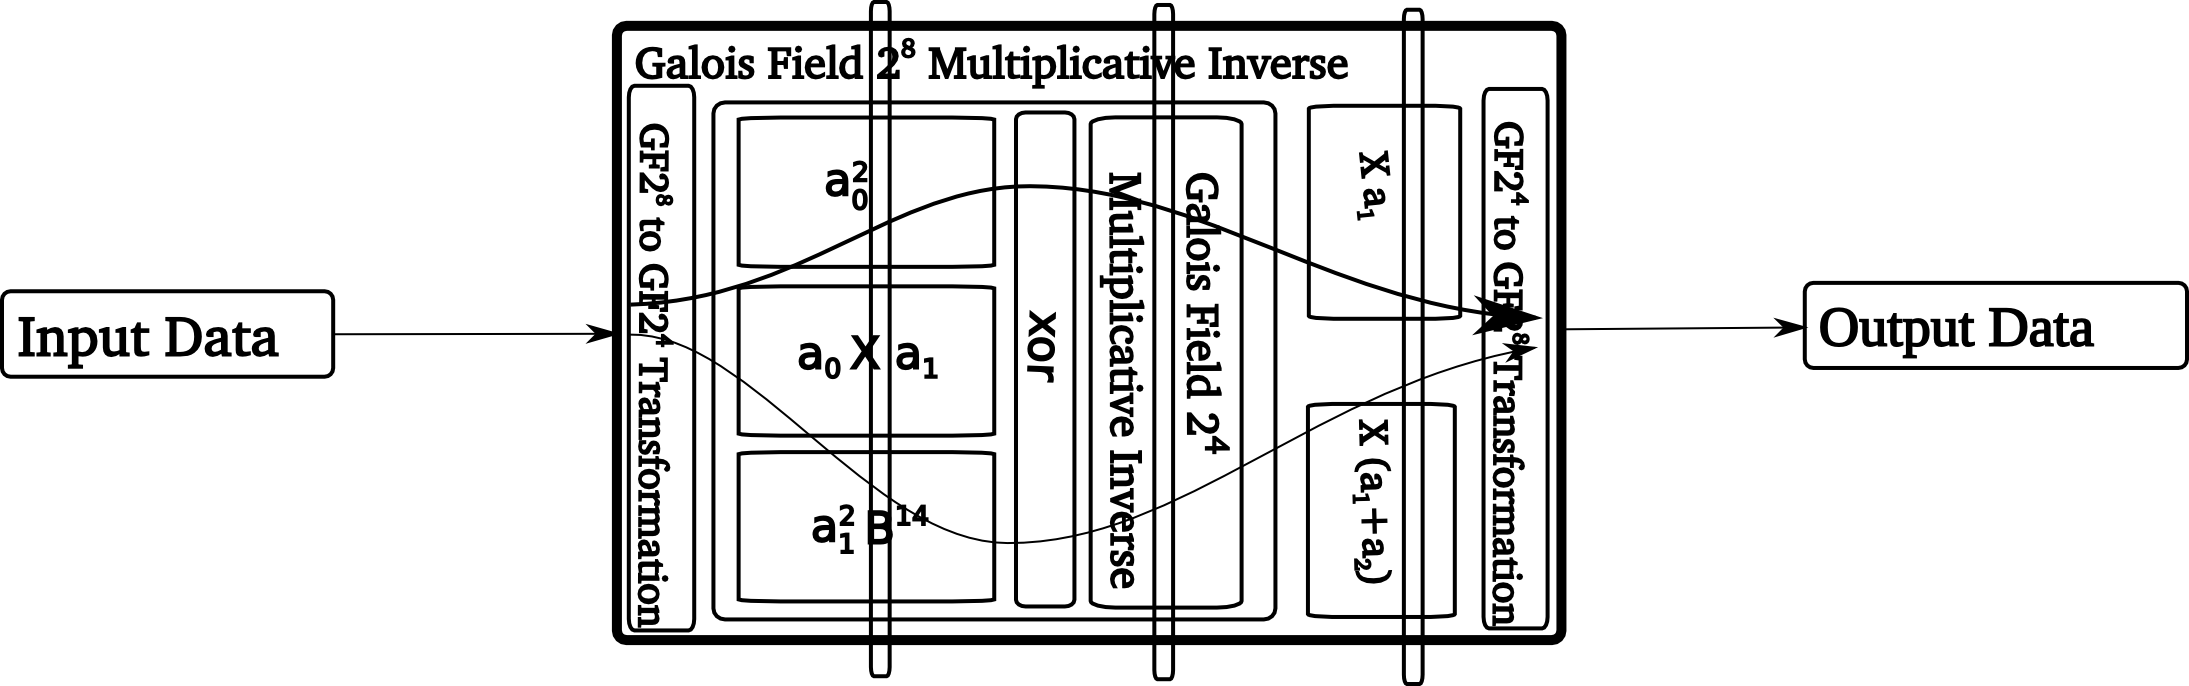
\includegraphics[width=0.50 \textwidth]{composite.png}
%\caption{GF $2^8$ inversion by using composite field}
%\label{composite}
%\end{figure}

\begin{figure}
\centering
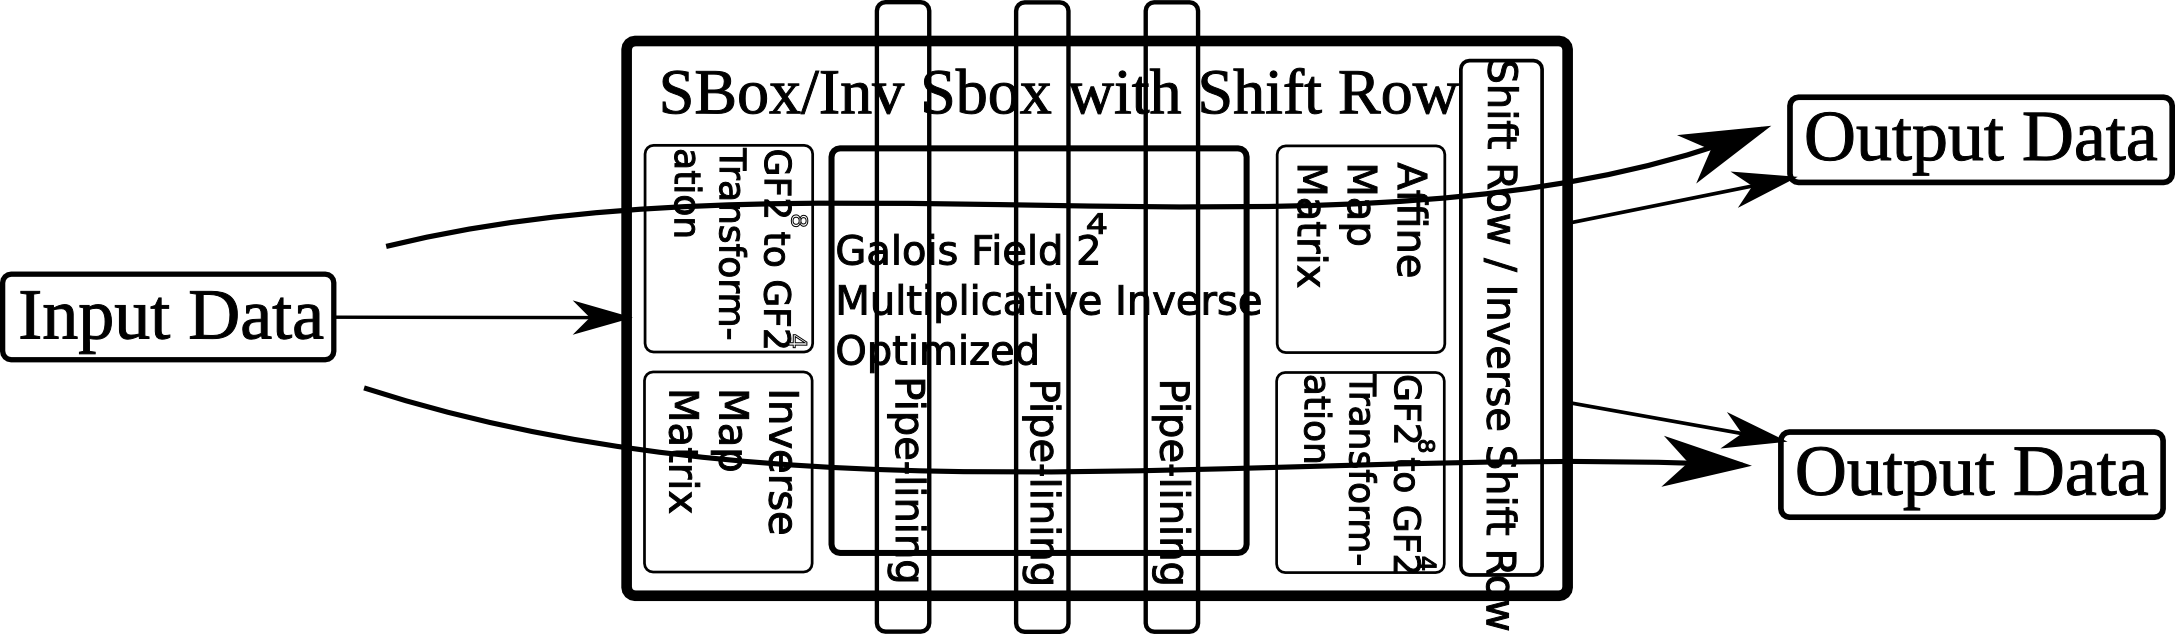
\includegraphics[width=0.50 \textwidth]{sbox.png}
\caption{Sbox module merged with shift module}
\label{Sbox}
\end{figure}

\section{ShiftRows Transformation}
\label{sec:shift}

In the ShiftRow transformation, the bytes in the last three rows of the State are cyclically shifted over different numbers of bytes (offsets). The first row, r = 0, is not shifted. Specifically, the ShiftRow transformation proceeds as follows:

\begin{equation}
s_{r,c}'~ = ~s_{r,(c+shift(r,Nb))mod Nb}  ~ for ~0<r<4~ and ~0\leq c <Nb~
\label{eq:sub3}
\end{equation}
where the shift value shift(r,Nb) depends on the row number, r, as follows (recall that Nb = 4): 
\begin{equation}
shift (1,4) = 1 ; shift (2,4) = 2 ; shift (3,4) = 3 
\label{eq:sub4}
\end{equation}
This has the effect of moving bytes to \textquotedblleft lower\textquotedblright  positions in the row (i.e., lower values of c in a given row), while the \textquotedblleft lowest\textquotedblright  bytes wrap around into the \textquotedblleft top\textquotedblright  of the row (i.e., higher values of c in a given row). 
Shift Row have been implemented with the help of bus multiplexers.

This process operates individually on rows with individual offset byte.  The transform throughput is 32 bits per clock cycle and can be pipelined for column order. For a wider data path (128-bit) or the higher throughput such as 128 bits per clock cycle, multiplexers are not necessary. In 128-bit design Shift Row is merged in the Substitution module. Refer to the (figure:\ref{Sbox}). Thus simplifying the design and eliminating some multiplexers and reducing the size.

\section{MixColumn Transformation\cite{1512188}}
\label{sec:mix}

The MixColumn transformation operates on the State column-by-column, treating each column as a four-term polynomial. The columns are considered as polynomials over $GF(2^8)$ and multiplied modulo $x^4 + 1$ with a fixed polynomial a(x), given by 
\begin{equation}
a(x) = \{03\}~x^3 ~+ ~\{01\}~x^2 ~+ ~\{01\}~x ~+ ~\{02\}
\label{eq:sub5}
\end{equation}

This can be written as a matrix multiplication. Let 

$s'(x) = a (x) \oplus s(x)~ :$ 
\begin{equation}
\left[ \begin{array}{c}
s_{0,c}' \\s_{1,c}' \\s_{2,c}' \\s_{3,c}' \end{array} \right] =
\left[ \begin{array}{cccccccc}
02 & 03 & 01 & 01\\
01 & 02 & 03 & 01\\
01 & 01 & 02 & 03\\
03 & 01 & 01 & 02\\
 \end{array} \right] \oplus
 \left[ \begin{array}{c}
s_{0,c}\\s_{1,c}\\s_{2,c}\\s_{3,c} \end{array} \right]
\label{eq:sub6}
\end{equation}

\subsection {InvMixColumn Transformation}
\label{sec:invmix}

InvMixColumn is the inverse of the MixColumns transformation. InvMixColumn operates on the State column-by-column, treating each column as a four-term polynomial. The columns are considered as polynomials over $GF(2^8)$ and multiplied modulo $x^4 + 1 $ with a fixed polynomial $a^{-1}(x)$, given by 
\begin{equation}
a^{-1}(x) = \{0b\}x^3 + \{0d\}x^2 + \{09\}x + \{0e\}
\end{equation}
this can be written as a matrix multiplication. Let 
$s'(x) = a^{-1}(x) \oplus s(x)~ :$
\begin{equation}
\left[ \begin{array}{c}
s_{0,c}' \\s_{1,c}' \\s_{2,c}' \\s_{3,c}' \end{array} \right] =
\left[ \begin{array}{cccccccc}
0e & 0b & 0d & 09\\
09 & 0e & 0b & 0d\\
0d & 09 & 0e & 0b\\
0b & 0d & 09 & 0e\\
 \end{array} \right] \oplus
 \left[ \begin{array}{c}
s_{0,c}\\s_{1,c}\\s_{2,c}\\s_{3,c} \end{array} \right]
\end{equation}

we can see that coefficients of $a^{-1}$ are more complex than coefficients of $a(X)$.As a result, hardware implementing AES decryption is larger and slower than for encryption. In order to reduce hardware cost, the InvMixColumn can be decomposed to share logic resources with MixColumn.

\subsection {MixColumn in sub galois field}
Since this math is done in Rijndael's Galois field, the MixColumn and InverseMixColumn can be transformed in the sub Galois Field same used in the subbyte.

For example MixColumn can be represented by

\begin{equation}
\left[ \begin{array}{c}
s_{0,c}' \\s_{1,c}' \\s_{2,c}' \\s_{3,c}' \end{array} \right] =
\left[ \begin{array}{cccccccc}
02 & 03 & 01 & 01\\
01 & 02 & 03 & 01\\
01 & 01 & 02 & 03\\
03 & 01 & 01 & 02\\
 \end{array} \right] \oplus
 \left[ \begin{array}{c}
s_{0,c}\\s_{1,c}\\s_{2,c}\\s_{3,c} \end{array} \right]
\end{equation}

now let's say $\delta$ is the transformation function for $GF(2^8) \rightarrow GF((2^4)^2)$ field transformation then

\begin{equation}
\delta \left(\left[ \begin{array}{c}
s_{0,c}' \\s_{1,c}' \\s_{2,c}' \\s_{3,c}' \end{array} \right]\right) =
\delta \left(\left[ \begin{array}{cccccccc}
02 & 03 & 01 & 01\\
01 & 02 & 03 & 01\\
01 & 01 & 02 & 03\\
03 & 01 & 01 & 02\\
 \end{array} \right]\right) \oplus
 \delta \left(\left[ \begin{array}{c}
s_{0,c}\\s_{1,c}\\s_{2,c}\\s_{3,c} \end{array} \right]\right)
\end{equation}

where mix column metrix in sub galois field (same field which have been used in subbyte) can be computed as

\begin{equation}
\delta \left(\left[ \begin{array}{cccccccc}
02 & 03 & 01 & 01\\
01 & 02 & 03 & 01\\
01 & 01 & 02 & 03\\
03 & 01 & 01 & 02\\
 \end{array} \right]\right) = \left[ \begin{array}{cccccccc}
2e & 2f & 01 & 01\\
01 & 2e & 2f & 01\\
01 & 01 & 2e & 2f\\
2f & 01 & 01 & 2e\\
 \end{array} \right]
\end{equation}


similarly inv mix column metrix in sub galois field can be computed as


\begin{equation}
\delta \left(\left[ \begin{array}{cccccccc}
0e & 0b & 0d & 09\\
09 & 0e & 0b & 0d\\
0d & 09 & 0e & 0b\\
0b & 0d & 09 & 0e\\
 \end{array} \right]\right) = \left[ \begin{array}{cccccccc}
24 & 6c & 0b & 42\\
42 & 24 & 6c & 0b\\
0b & 42 & 24 & 6c\\
6c & 0b & 42 & 24\\
 \end{array} \right]
\end{equation}

now we may find a sub field for which these metrices may result in better optimised for implementation point of view then we can do all the rounds in same sub galois field. And do the GF transformations at the last and at the end. That way we can better optimise the implementation.

\bibliography{thesis}
\bibliographystyle{ieeetr}

\end{document}
